\documentclass{article}
\usepackage[utf8]{inputenc}
\usepackage{graphicx}
\usepackage{float}

\title{COL380: Assignment 1}
\author{Sachin 2019CS10722 }
\date{January, 2022}

\begin{document}

\maketitle

\section{Implementation}
I've followed the steps provided in the document to implement parallel sort algorithm using tasks. 
The psuedo code is as follows:- 

\begin{enumerate}
    \item \textbf{Algorithm: }

algorithm parallerSort(data,n,p):\\
\hspace*{0.5cm}if ($p*p > n$) then do sequentialSort(data,n)\\
\hspace*{0.5cm}else do\\
\hspace*{1cm}threshold = $2*n/p$\\
\hspace*{1cm}create array R of size $p*p$\\
\hspace*{1cm}from each p size bucket of data add first p elements in R\\
\hspace*{1cm}sort R\\
\hspace*{1cm}create array S of size p+1\\
\hspace*{1cm}$S[0] = -inf$\\
\hspace*{1cm}for i = 0 to p-1 do $S[i+1] = R[(i+1)*p]$\\
\hspace*{1cm}$S[p] = inf$\\
\hspace*{1cm}delete R;\\
\hspace*{1cm}create 2d array B of size $p*n$\\
\hspace*{1cm}create array Bsize that stores size of each bucket in B\\
\hspace*{1cm}for i = 0 to p-1 do\\
\hspace*{1.5cm}create a task with B, Bsize shared and i private\\
\hspace*{1.5cm}assign task to find elements of data data such that:\\
\hspace*{2cm}$S[i] < data[j] \& data[j] \leq S[i+1]$\\
\hspace*{1.5cm}add satisfied elements to $B[i]$\\
\hspace*{1.5cm}if $B[i].size > threshold$ do parallerSort(B[i])\\
\hspace*{1.5cm}else do sequentialSort(B[i])\\
\hspace*{1cm}wait for all tasks to complete\\
\hspace*{1cm}for i = 0 to p-1 do\\
\hspace*{1.5cm}create a task with B, Bsize shared and i private\\
\hspace*{1.5cm}add elements of $B[i]$ at correct position in data\\
\hspace*{1cm}wait for all tasks to complete\\
\hspace*{1cm}delete S, B, Bsize\\

So, basically for the case of tasks I've created p tasks that find the elements that lie in ith 
partition in O(n) pass of array and finally wait for all tasks to complete then add the sorted partitions
back to data by creating p tasks again. 

\item \textbf{Design Choices: }

\begin{enumerate}
    \item I've used quick sort as sequential sort algorithm.
    \item I've created p independent tasks that have independent job of finding elements lying in ith partition.
        This makes mutual exclusion between tasks simpler and cache friendly.\\
        But this has one disadvantage that it will only require max p cpu to work upon, if more that p cpu are provided 
        this will Implementation will not use them.
    \item Initially we do not know the size of each partition, so I have assigned it to be size and increment atcual size every time an 
    element is added, this will require high space requirenment (linear in n) and better algorithms are proposed but they require inter task
    communication (basically each task send their element to a central task that adds that element in data directly) but we do not have any concrete way
    of inter task communication.

\end{enumerate}

\end{enumerate}



\section{Results}


\begin{enumerate}
    \item \textbf{input size = $2^{25}$: }
    
    Since, input size $2^{32}-1$ was taking too much of time (around 3 hours to run for 15 iterations of varying number of threads) 
    so I did my rigrous testing on input size $2^{25}$ and on input size $2^{32}-1$ just plotted the final graph.
    
    \begin{enumerate}

        \item \textbf{Number of cpu vs runtime:- }
        
        I plotted time taken by algorithm to sort array of size $2^{25}$ by varying number of cpu with number of threads and p kept constant. 
        (part of analysis that was mentioned in pdf provided) and result is shown on next page:- 

        Clearly time reduces on increasing number of cpu, hence algorithm scales with number of cpu.\\
        However, this graph shows the scalability of algorithm but there are other subtleties that need to 
        seen like how algorithm on varying other parameters like number of threads used and number of buckets(p). Lets see
        those behaviour.

        \begin{figure}[H]
            \centering
            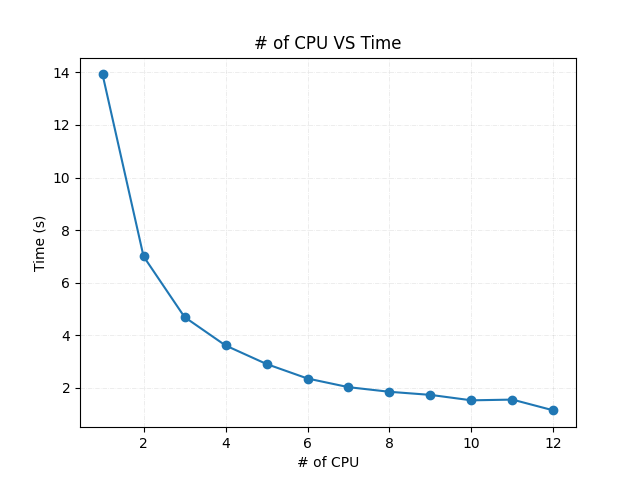
\includegraphics[width=10cm]{../graph.png}
            \caption{\# of cpu vs time}
        \end{figure}


        \item \textbf{Number of threads vs runtime: Varying p:- }
        In this part of testing I tried varying p with number of cpu set constant as 5.
        Here are the results:- 

        \begin{figure}[H]
            \centering
            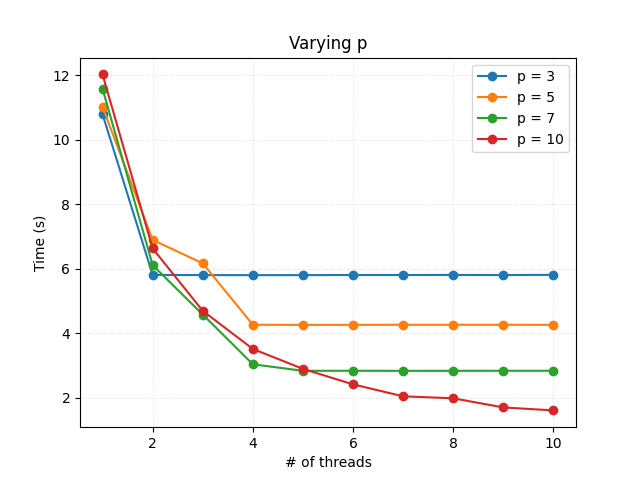
\includegraphics[width=10cm]{../varyingp.png}
            \caption{\# threads vs time with varying p}
        \end{figure}

        Clearly, on increasing number of threads, time taken by algorithm reduces (that is what is expected) as more the number of threads, 
        tasks can be assigned to their own threads and less sharing of threads by tasks (that first of all directly reduces time as now more number of 
        tasks as running parallely and also secondrarily it reduces scheduling overhead).\\
        But, there is a catch here. For p = k, time only reduces untill number of threads = k. After that time more or less remains constant (for all values 
        of p) this is because our tasks are bounded by p. And increasing number of threads beyound p should'nt have any effect on runtime as only p threads are going to 
        be used eventually.
        
        \item \textbf{Number of threads vs runtime: Varying no of of cpu:- }
        
        For this part I've plotted varying time with number of threads for different number of cpu. Value of p is kept constant = 24. \\

        \begin{figure}[H]
            \centering
            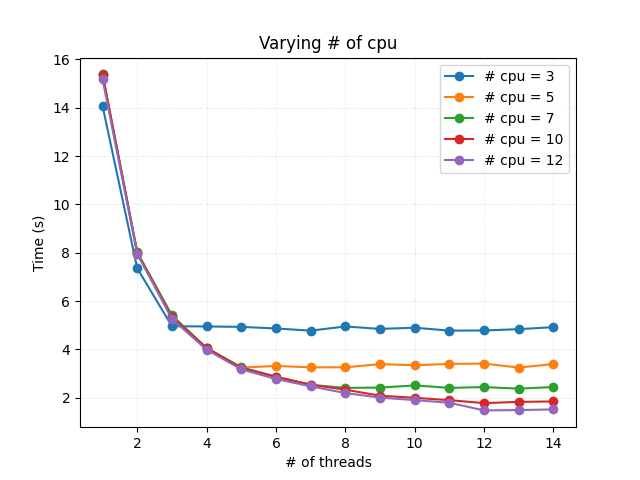
\includegraphics[width=10cm]{../varyingc.png}
            \caption{\# threads vs time with varying no of cpu}  
        \end{figure}

        This graph again shows that increasing number of threads reduces runtime of algorithm. But only upto number of threads equal to number of cpu provided 
        after that time remains more or less constant (somtimes increases a bit)\\
        This is because if number of threads are less than number of cpu then each thread will get its own cpu and tasks will run parallely on different cpu. But as soon as 
        number of threads become more than number of cpu, few threads will share same cpu and hence have to be scheduled hence in effect only c (number of cpu) threads are
        running parallely at any point of time. Hence time remains constant.


    \end{enumerate}

    \item \textbf{input size = $2^{32}$: }
    
    I then tested my code on the maximum possible input size = $2^{32}-1$ and plotted runtime vs number of cpu and here are the results.
    \begin{figure}[H]
        \centering
        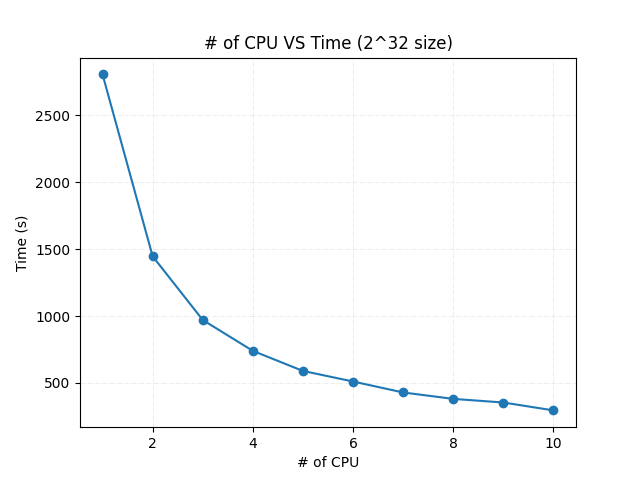
\includegraphics[width=10cm]{../graph32.png}
        \caption{\# threads vs time with varying no of cpu}
    \end{figure}

    Clearly algorithm runtime decreases.\\

    \textbf{NOTE: }In this part i limited number of cpu to 10 only because I was not able to get 12 cpu job run on hpc (its in queue for 1 day as of now and not yet started).

\end{enumerate}


\end{document}
